\documentclass[12pt,addpoints,answers]{exam}
\usepackage[utf8]{inputenc}

\unframedsolutions
\renewcommand{\solutiontitle}{\noindent\textbf{Solution:}\par\noindent}
\SolutionEmphasis{\color{blue}}
\printanswers

\usepackage{booktabs}
\usepackage{tabularx}
\usepackage{xfrac}

\usepackage{siunitx}
\sisetup{parse-numbers=false}

\usepackage{listings}
\lstset{basicstyle=\scriptsize\ttfamily}

\usepackage{tikz}
\usetikzlibrary{arrows}
\usetikzlibrary{decorations.pathreplacing}
\usetikzlibrary{chains}
\usetikzlibrary{positioning}
%\tikzset{>=stealth',every on chain/.append style={join}, every join/.style={-,blue,thick,dashed}}



\title{Computer Networks Homework 1}
\author{Fall 2019}
\date{Due: 3 February 2020}

\begin{document}
\maketitle

\begin{questions}
\question[12] Imagine that there are two paths a packet could take to travel from Host $J$ to Host $K$, as illustrated here:
\begin{center}
	Minor fix, we're assuming $(Host A = Host J)$ and $(Host B = Host K)$
\end{center}
\begin{center}
\begin{tikzpicture}[
	node distance=1.00in
]
\node[label=below:{\scriptsize{Host A}}]                                          (hostA)     {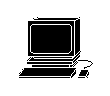
\includegraphics[scale=0.5]{fig/cisco/workstation}};
\node[label=above:{\scriptsize{Switch}}, right of=hostA]                          (switchA.1) {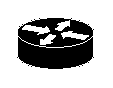
\includegraphics[scale=0.5]{fig/cisco/router}};
\node[label=above:{\scriptsize{Switch}}, right of=switchA.1, node distance=1.5in] (switchA.2) {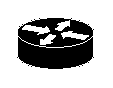
\includegraphics[scale=0.5]{fig/cisco/router}};
\node[label=above:{\scriptsize{Switch}}, right of=switchA.2, node distance=1.5in] (switchA.3) {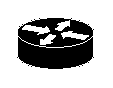
\includegraphics[scale=0.5]{fig/cisco/router}};
\node[label=below:{\scriptsize{Switch}}, below of=switchA.1, node distance=0.5in] (switchB.1) {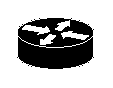
\includegraphics[scale=0.5]{fig/cisco/router}};
\node[label=below:{\scriptsize{Switch}}, right of=switchB.1]                      (switchB.2) {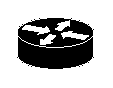
\includegraphics[scale=0.5]{fig/cisco/router}};
\node[label=below:{\scriptsize{Switch}}, right of=switchB.2]                      (switchB.3) {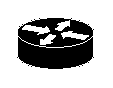
\includegraphics[scale=0.5]{fig/cisco/router}};
\node[label=below:{\scriptsize{Switch}}, right of=switchB.3]                      (switchB.4) {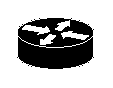
\includegraphics[scale=0.5]{fig/cisco/router}};
\node[label=below:{\scriptsize{Host B}}, right of=switchA.3]                      (hostB)     {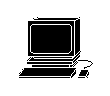
\includegraphics[scale=0.5]{fig/cisco/workstation}};
\begin{scope}[start chain,>=stealth',every on chain/.append style={join}, every join/.style={-,blue,thick,dashed}]
	\chainin (hostA);
	\chainin (switchA.1);
	\chainin (switchA.2);
	\chainin (switchA.3);
	\chainin (hostB);
\end{scope}
\begin{scope}[start chain,>=stealth',every on chain/.append style={join}, every join/.style={-,red,thick}]
	\chainin (switchA.1);
	\chainin (switchB.1);
	\chainin (switchB.2);
	\chainin (switchB.3);
	\chainin (switchB.4);
	\chainin (switchA.3);
\end{scope}
\end{tikzpicture}
\end{center}
Each link drawn with a dashed blue line has a bandwidth of \SI{250000}{bps}; each link drawn with a solid red line has a bandwidth of \SI{400000}{bps}. Packets are always \SI{1000}{bytes}. You may assume that process, queue, and propegation delays are negligable.

What is the delay in each path? Which path should the packet take to get to Host $K$ the fastest?

\begin{solution}
		Since only a single packet is specified and only transmission delays are non negligable calculating the two paths is simply calculating the total transmission delay on both routes.

	Transmission delay is defined as $D_t = N / R$ where:
	\begin{enumerate}
		\item $D_t$ = the transmission delay in seconds
		\item $N$ = the number of bits
		\item $R$ = the rate of transmission in bps.
	\end{enumerate}

	Our total payload is one packet of size 1000 bytes (8000 bits).

	The delay from one computer (host or switch) to another is $8000 / 250000 = 0.032$ seconds on the blue line.

	The delay from one computer (host or switch) to another is $8000 / 400000 = 0.02$ seconds on the red line.

	The path along the exclusively blue line contains 4 hops leading us to an easy $0.032 * 4 = 0.128$ seconds

	The other path contains two blue hops and 5 red hops.  So, $0.032 * 2 = 0.064$ seconds on the blue hops, and $0.02 * 5 = 0.16$ seconds on the red hops.  Combining these gives us a total of $0.064 + 0.16 = 0.224$ seconds on the secondary path.

	From this, we can state that the packet should take the exclusively blue line to send the packet with the lowest latency.
\end{solution}
\begin{center}
	Solution 1
\end{center}
\begin{flushleft}

\end{flushleft}

\question[8] Consider again the network in Question 1. Each link drawn with a dashed blue line still has a bandwidth of \SI{250000}{bps}. What is the minimum bandwidth for solid red links such that the bottom path is faster than the top path?

\begin{solution}
	In short, the minimum amount of bandwidth required to ensure that the exclusive blue line has a lower latency than the red line is when the exclusively blue line is over saturated.  This happens with an average throughput of \SI{250000}{bps}, so the volume of traffic where the exclusively blue line is saturated is at least \SI{250001}{bps}.
\end{solution}

\question[12] A mountain bike rider is competing in the Tour Divide, a \SI{4418}{\kilo\meter} race from Banff, Alberta to Antelope Wells, New Mexico. She is carrying a GPS tracker, as do all racers. The tracker sends a signal to a satellite, which relays it back down to a server in New Orleans, LA. A friend of this rider wants to know her current position. What is the delay from when the signal leaves the tracker to when the friends computer in Seattle, Washington?

Assume the following:
\begin{enumerate}
\item the connection from the tracker to the satellite (and the satellite back to the server) is wireless and the signal travels at the speed of light,
\item the satellite is orbiting in medium-Earth orbit at approximately \SI{20000}{\kilo\meter},
\item the friend is using a copper connection to retieve the information,
\item it is approximately \SI{4228}{\kilo\meter} from New Oreleans to Seattle, and finally,
\item the transmission delay of the packet of the packet is negligible because it is so small.
\end{enumerate}
\begin{solution}
	\begin{enumerate}
		\item First is calculating the latency from the tracker to the satellite (hop 1 to 2).  The speed of light is 299792 km/s, over a distance of 20000 km.  This gives us $20000 km / 299792 (km/s) = 0.066712921$ seconds.  This is then doubled from $0.066712921$ seconds to $0.13342584$ to account for bouncing back to the server in New Orleans. for the transmission delay.
		
		\item Second is calculating the hop from the server to the friends computer in Seattle.  The propagation speed of copper cable is $2.3 * 10^8$ m/s from the given slides.  Converting $4228$ km to meters gives us $4228000$.  From here, we can calculate the latency with $4228000/(2.3 * 10^8) = 0.018382609$ seconds.
		
		\item Combining these together we get a transfer speed of $0.13342584 + 0.018382609 = 0.15180845$ seconds, or more commonly:$151.80845$ ms. 
	\end{enumerate}
\end{solution}

\question[12] A security camera captures images that are each \SI{100000}{bytes} in size. It takes one image every \SI{.25}{\second}. If there is a \SI{500}{\meter} point-to-point (cable, $\SI{2.3 \cdot 10^8}{bps}$ propegation rate) connection to the monitor where the security guard inspects these images, what is the minimum acceptable bandwidth (bandwidth required to transmit one image before the next is taken) between the camera and monitor?
\begin{solution}
	\begin{enumerate}
		\item First we convert $100000$ bytes to bits -> $800000$ bits.
		
		\item Second figure out the potential throughput by dividing $500$m by $2.3 * 10^8$ equaling $0.000002173913$ capability of a moment on the line.
		
		\item The minimum bandwidth needs to be capable of dealing with $800000$ bits per image four times a second, meaning $3200000$ bits.
		
		\item $3200000$ bit of images per second across a line of $0.000002173913$, multiplying together getting a required bandwidth of $6.9565216$ bps.
	\end{enumerate}
	%This number does not look right, but I can't figure out why.  I recoworked the equation in 3 ways and it's still like this.
\end{solution}

\question[8] A standard Ethernet frame (or packet) is \SI{1500}{bytes}. The most common version of Ethernet found on consumer devices is Gigabit Ethernet, which operates with a bandwidth of \SI{1}{Gbps}. If two hosts are placed \SI{2500}{\meter} away from each other, how many frames should be sent out to ``peek the pipe full'' for the full Round Trip Time?
\begin{solution}
	\begin{enumerate}
		\item Consumer devices usually run on copper cabling with a propagation rate of $2.3 * 10^8$ m/s.  Across a range of 2500m, doubled to 5000m for round trips is $0.00002173913$ seconds for a round trip.
		
		\item Since we're dealing with round trip traffic, we can essentially slice the bandwidth in half for our calculations (half up half down).  Giving us $500$ Mbp/s ($500000$ bp/s) of traffic to saturate, given $12000$ bits per packet.  It will take $41 \frac{2}{3}$ packets to statically saturate the line, which we'll round up to $42$.
		
		\item Since traffic is constantly going on and off the line the transmission delay is $\frac{data}{bps}$ is $\frac{42}{0.00002173913}$ which is $1932000$ packets to saturate the line.
	\end{enumerate}
% that equates to like 3 gb/s of traffic??? this can't be right.
\end{solution}

\question Let's think a little about security in my analogy of sending a multi-part present to Samantha. Suggest mechanisms to accomplish each of the following tasks below. Remember that we are protecting physical packages, not packets!
\begin{parts}
\part[4] I don't want the post office to know who the source of the presents is, but I want Samantha and her mom to know.
\part[4] I don't want anybody except Samantha to know who the source of the presents is.
\part[4] Even if the postal worker opens up the packages, I don't wnat him to know that the three packages are related.
\end{parts}
\begin{solution}
	\begin{enumerate}
		\item To solve (a) the answer is to not provide a return address on the box, but leave a note saying who it was from inside the box.
		
		\item To solve (b) Put a box inside of a box, where the outside box has only a mailing address to Samantha's mom.  The inside box should have a label on it saying for Samantha, and then a note inside the inner box that says who it is from.
		
		\item Assuming the postal worker only opens up the outer package, the method from solution (b) would solve this, with the addition of putting the package number inside a slip in the inner box.
	\end{enumerate}
\end{solution}

\question[8] A standard Ethernet frame has a payload of \SI{1500}{octets}. I have designed an application-layer protocol with a fixed 16 octets of header data. Use any reliable resource to find the standare header sizes for TCP and IP. What is the maximum actual data that can fit into the payload of that Ethernet frame after all the headers? What is the percentage overhead?
\begin{solution}
	The maximum size of a TCP header is $60$ bytes (minumum of $20$ bytes) and the maximum size of the packet is $65535$ bytes.  The $16$ octet header conveniently falls at the required $32$ bit boundary defined, however is not at the required minimum header size of $20$ bytes so we have $4$ bytes of zero padding.
	
	The maximum actual data that may fit in is $1500 - 20 = 1480$ bytes of data.
	
	Overhead can be calculated with the following:
	\begin{center}
		$\frac{Packet Size - Payload Size}{Packet Size}$
	\end{center}
	For us this is $\frac{1500 - 1480}{1500}$, which gives us a protocol overhead of $0.013333333 \%$.
\end{solution}

\question[8] Shown below is a simple HTTP GET request with some cookie values. What is the ultimate address that is requested by the client? (You may have to make some assumptions about how the server interprets the cookies. State these assumptions and make them logical!)\\
\begin{minipage}{\textwidth}
\begin{lstlisting}[language={},escapechar=§,basicstyle=\ttfamily,breaklines=true]
GET /pages/home.html HTTP/1.1
Host: www.mtu.edu
Connection: close
User-Agent: Mozilla/5.0 (Macintosh; Intel Mac OS X 10_14_6) AppleWebKit/537.36 (KHTML, like Gecko) Chrome/76.0.3809.132 Safari/527.36
Cookie: user=newton
Cookie: dept=ECE
Cookie: userprefixchar=%7E
\end{lstlisting}
\end{minipage}
\begin{solution}
	The web URL being accessed is $https://www.mtu.edu/pages/home.html$.
	
	MTU enforces a redirect policy on non SSL/TLS traffic to SSL/TLS (https), since the header doesn't make any note of HSTS it's likely a normal Apache rewrite rule.  
	
	Appending the GET location to Host is rather obvious, I think the only really tricky thing in this problem is the Cookie sections.  However, they are meant to stay in the header, and not be added to the URL.  While you technically could pass and parse cookies along the URL as part of a $?key=value;$ (similar to that PHP uses) it's considered rather insane to do so.  Cookies tend to store private information and should be handled over encrypted traffic (in the header).  The URL sent out in plain text so it knows where to go.
\end{solution}

\question[8] Show a full HTTP response message for a simple HTML document that just has the text, ``Hello, World!'' as its sole content. Send two cookies to the client: a random session key called PersonID; and a cookie called Planet with the value ``Earth'' that expires on January 1, 2099 at 11:59 pm.
\begin{solution}
	\begin{minipage}{\textwidth}
		\begin{lstlisting}[language={},escapechar=§,basicstyle=\ttfamily,breaklines=true]
			HTTP/1.1 200 OK
			Date: Mon, 3 Feb 2020 12:28:53 GMT
			Server: Apache/2.2.14 (Win32)
			Last-Modified: Mon, 22 Feb 2020 19:15:56 GMT
			Set-Cookie: PersonID="randomSessionKey"
			Set-Cookie: Planet="Earth";  Expires=1 Jan 2099 11:59:00 GMT
			Content-Length: 31
			Content-Type: text/html
			Content:
			
			<html>
			Hello, World!
			</html><cr><lf>
		\end{lstlisting}
	\end{minipage}
\end{solution}

\question[12] A somewhat smart browser makes an initial request for a webpage an closes the connection. After parsing the requested page, it will make several consecutive requests for the images without closing the connection. If the webpage below shows the HTML page requested by the original request, show the subsequent request and response messages. You do not need to make up data for the images, but get the Content Type correct!\\
\begin{minipage}{\textwidth}
\begin{lstlisting}[language={},escapechar=§,basicstyle=\ttfamily,breaklines=true]
<HTML>
  <HEAD>
    <TITLE>My Vacation Pictures</TITLE>
  </HEAD>
  <BODY>
    <H1>Pictures from my vacation to Japan!</H1>
    <IMG src=GoldenPavillion.png>
    <br>
    <IMG src=food.jpg>
    <br>
    <IMG src=Geisha.png>
    <br>
  <BODY>
</HTML>
\end{lstlisting}
\end{minipage}

\begin{solution}
	
	% Golden Pavillion.png
	Golden Pavillion GET
	\begin{minipage}{\textwidth}
	\begin{lstlisting}[language={},escapechar=§,basicstyle=\ttfamily,breaklines=true]
	GET /GoldenPavillion.png HTTP/1.1
	User-Agent: Mozilla/4.0 (compatible; MSIE5.01; Windows NT)
	Host: www.tutorialspoint.com
	Accept-Language: en-us
	Accept-Encoding: gzip, deflate
	Connection: Keep-Alive
	\end{lstlisting}
\end{minipage}

	Golden Pavillion Response
	\begin{minipage}{\textwidth}
	\begin{lstlisting}[language={},escapechar=§,basicstyle=\ttfamily,breaklines=true]
	HTTP/1.1 200 OK
	Date: Mon, 3 Feb 2020 19:15:56 GMT
	Server: Apache/2.2.14 (Win32)
	Last-Modified: Mon, 22 Feb 2020 19:15:56 GMT
	Content-Length: someNumberInBytes
	Content-Type: text/html
	Content: image/png
	
	<image data><cr><lf>
	\end{lstlisting}
	\end{minipage}

	% food.jpg
	food GET
\begin{minipage}{\textwidth}
	\begin{lstlisting}[language={},escapechar=§,basicstyle=\ttfamily,breaklines=true]
	GET /food.png HTTP/1.1
	User-Agent: Mozilla/4.0 (compatible; MSIE5.01; Windows NT)
	Host: www.tutorialspoint.com
	Accept-Language: en-us
	Accept-Encoding: gzip, deflate
	Connection: Keep-Alive
	\end{lstlisting}
\end{minipage}

	food Response
\begin{minipage}{\textwidth}
	\begin{lstlisting}[language={},escapechar=§,basicstyle=\ttfamily,breaklines=true]
	HTTP/1.1 200 OK
	Date: Mon, 3 Feb 2020 19:15:56 GMT
	Server: Apache/2.2.14 (Win32)
	Last-Modified: Mon, 22 Feb 2020 19:15:56 GMT
	Content-Length: someNumberInBytes
	Content-Type: image/jpeg
	Content:
	
	<image data><cr><lf>
	\end{lstlisting}
\end{minipage}

	% Geisha
	Geisha GET
\begin{minipage}{\textwidth}
	\begin{lstlisting}[language={},escapechar=§,basicstyle=\ttfamily,breaklines=true]
	GET /Geisha.png HTTP/1.1
	User-Agent: Mozilla/4.0 (compatible; MSIE5.01; Windows NT)
	Host: www.tutorialspoint.com
	Accept-Language: en-us
	Accept-Encoding: gzip, deflate
	Connection: Keep-Alive
	\end{lstlisting}
\end{minipage}

	Geisha Response
\begin{minipage}{\textwidth}
	\begin{lstlisting}[language={},escapechar=§,basicstyle=\ttfamily,breaklines=true]
	HTTP/1.1 200 OK
	Date: Mon, 3 Feb 2020 19:15:56 GMT
	Server: Apache/2.2.14 (Win32)
	Last-Modified: Mon, 22 Feb 2020 19:15:56 GMT
	Content-Length: someNumberInBytes
	Content-Type: image/png
	Content:
	
	<image data><cr><lf>
	\end{lstlisting}
\end{minipage}
\end{solution}

\end{questions}
\end{document}
